% Source printed pp. 279-292 / PDF pp. 287-300.
\section{Mumford 与 Gieseker 的射影性证明}\label{src:6.8}
\begin{epigraph}
毫不夸张地说, [定理 A] 在过去三十年的代数曲线理论中所起的基础性作用, 可与抽象曲线理论在此前六十年中的作用相比.
\epigraphauthor{Joe Harris 和 Ian Morrison~\cite[48 页]{HM98}}
\end{epigraph}
Mumford 在~\cite{GIT} 中发展几何不变量理论 (GIT), 用以构造代数几何中的商与模空间. 核心思想是将模叠 $\mathcal M$ (如 $\overline{\mathcal M}_g$) 表示为商叠 $[U/G]$, 其中 $G$ 约化, $U\subseteq\mathbb P(V)$ 为 $G$-表示 $V$ 的射影化的局部闭子概形, 并用 Hilbert--Mumford 判据 (\bookref{8.4.4}) 证明 $u\in\overline U$ 属于 $U$ 当且仅当它 GIT 稳定. 有趣的是, Mumford 首次将 $M_g$ 构造为 $\mathbb Z$ 上概形~\cite[定理 5.11, 7.13]{GIT}, 所用的是针对性技巧. 不久后, Mumford~\cite{Mum77} 和 Gieseker~\cite{Gie82} 用 GIT 将 $\overline M_g$ 构造为射影簇. 但 $\overline M_{g,\allowbreak n}$ 射影性的首个证明由 Knudsen 和 Mumford~\cite{KM76,Knu83a,Knu83b} 给出, 依赖到主极化阿贝尔簇模空间的 Satake 紧化的 Torelli 映射 $\overline M_g\to\overline A_g$.

本节在特征 $0$ 代数闭域 $k$ 上\footnote{构造如何推广到正特征和混合特征, 见注记~\bookref{6.8.7}.}, 将第~\bookref{8} 章发展的 GIT 应用于 Chow 概形和 Hilbert 概形, 介绍 Mumford 构造 $\overline M_g$ 的方法.
\subsection{利用 Chow 与 Hilbert 概形的 GIT 纲要}\label{src:6.8.1-subsection}
Hilbert 概形的 GIT 构造依赖两个整数, Chow 概形的构造只依赖 $k$:
\begin{itemize}
\item $k\geq5$, 定义多重典范嵌入的对偶化层倍数:
\[
|\omega_C^{\otimes k}|:C\hookrightarrow\mathbb P^{N_k},\qquad N_k=(2k-1)(g-1)-1.
\]
需要 $k\geq3$, 使稳定曲线 $C$ 的 $\omega_C^{\otimes k}$ 丰沛; 需要 $k\geq5$, 才使 Chow 或 Hilbert 概形的 GIT 构造给出 $\overline M_g$.
\item $m\gg0$, 将 $k$-典范嵌入曲线的 Hilbert 概形嵌入 Grassmann 簇所用方程的次数. 为得到嵌入, 需要 $m\gg0$.
\end{itemize}
\noindent\textbf{Hilbert 概形.} 对 $k>1$, 亏格 $g$ 的 $k$-多重典范嵌入稳定曲线的 Hilbert 多项式为 $P(t)=\chi(C,\allowbreak \omega_C^{\otimes kt})=(2kt-1)(g-1)$. Hilbert 概形 $\operatorname{Hilb}^P(\mathbb P^{N_k})$ 在 $k$ 上射影 (定理~\bookref{2.1.2}), 带 $\operatorname{PGL}_{N_k+1}$ 作用. 对 $k\geq3$, 有不变局部闭子概形 $U$, 使 $\overline{\mathcal M}_g\cong[U/\operatorname{PGL}_{N_k+1}]$ (习题~\bookref{6.4.17}). 令
\begin{equation}\label{src:6.8.1}
H:=\overline U\subseteq\operatorname{Hilb}^P(\mathbb P^{N_k}).
\end{equation}
由定理~\bookref{2.4.5}, 对 $m\gg0$, 有等变闭浸入
\[
\begin{aligned}
H&\hookrightarrow\operatorname{Gr}(P(m),\Gamma(\mathbb P^{N_k},\mathcal O(m))),\\
[C\subseteq\mathbb P^{N_k}]&\mapsto[\Gamma(\mathbb P^{N_k},\mathcal O(m))\twoheadrightarrow\Gamma(C,\mathcal O(m))].
\end{aligned}
\]
其中左方截面空间为 $\operatorname{Sym}^m\Gamma(C,\allowbreak \omega_C^{\otimes k})$, 若 $C\in U$, 右方为 $\Gamma(C,\allowbreak \omega_C^{\otimes mk})$. 由命题~\bookref{2.2.8}, Plücker 嵌入为
\[
\begin{aligned}
\operatorname{Gr}(P(m),\Gamma(\mathbb P^{N_k},\mathcal O(m)))&\hookrightarrow\mathbb P\Bigl(\bigwedge^{P(m)}\Gamma(\mathbb P^{N_k},\mathcal O(m))\Bigr),\\
[\Gamma(\mathbb P^{N_k},\mathcal O(m))\twoheadrightarrow\Gamma(C,\mathcal O(m))]
&\mapsto\Bigl[\bigwedge^{P(m)}\Gamma(\mathbb P^{N_k},\mathcal O(m))\twoheadrightarrow\bigwedge^{P(m)}\Gamma(C,\mathcal O(m))\Bigr].
\end{aligned}
\]
事实上, 对任意 $\operatorname{Hilb}^P(\mathbb P^n)$, $m\gg0$ 时有 $\operatorname{PGL}_{n+1}$-等变闭浸入
\[
\operatorname{Hilb}^P(\mathbb P^n)\hookrightarrow\operatorname{Gr}(P(m),\Gamma(\mathbb P^n,\mathcal O(m)))
\hookrightarrow\mathbb P\Bigl(\bigwedge^{P(m)}\Gamma(\mathbb P^n,\mathcal O(m))\Bigr).
\]
研究不必多重典范嵌入的曲线的稳定性同样容易. 令 $\mathcal O_{\operatorname{Gr}}(1)$ 为 Grassmann 簇上的甚丰沛线丛, 令 $L_m=\mathcal O_{\operatorname{Gr}}(1)|_{\operatorname{Hilb}^P(\mathbb P^n)}$. 注意它依赖 $m$. 对 $m\gg0$, $L_m$ 甚丰沛, 继承 $\operatorname{PGL}_{n+1}$ 作用, 因而也继承 $\operatorname{GL}_{n+1}$ 和 $\operatorname{SL}_{n+1}$ 作用. 稍后限制到 $\operatorname{SL}_{n+1}$ 的单参数子群, 但同时考虑 $\lambda=\operatorname{diag}(\lambda_i)$, $\sum\lambda_i\ne0$ 也有用.
\begin{definition}\label{src:6.8.2}
对单参数子群 $\lambda:\mathbb G_m\to\operatorname{GL}_{n+1}$, 将 $[C\subseteq\mathbb P^n]$ 的 Hilbert--Mumford 指数 (定义~\bookref{8.4.1}) 记为 $\mu_{L_m}^{\mathrm{Hilb}}(C,\allowbreak \lambda)$.
\end{definition}
单项式 $x_0^{m_0}\cdots x_n^{m_n}$ 的 $\lambda$-权为 $\sum_i m_i\lambda_i$, 多项式的 $\lambda$-权为其中单项式的最大权. 对多项式集 $\beta=\{f_1,\allowbreak \ldots,\allowbreak f_p\}$, 记其权为各多项式权之和. 以下将 $\lambda$-权简记为 $\operatorname{wt}_\lambda$. 有
\begin{equation}\label{src:6.8.3}
\mu_{L_m}^{\mathrm{Hilb}}(C,\lambda)=\min_\beta\operatorname{wt}_\lambda(\beta),
\end{equation}
其中 $\beta\subseteq\Gamma(\mathbb P^n,\allowbreak \mathcal O_{\mathbb P^n}(m))$ 映到 $\Gamma(C,\allowbreak \mathcal O_C(m))$ 的基.

\noindent\textbf{Chow 概形.} 次数 $d$ 的整曲线 $C\subseteq\mathbb P^n$ 的 Chow 形式 $f_C\in\operatorname{Sym}^d(k^{n+1})^{\otimes2}$ 定义于~\bookref{2.4.5-subsection} 节. 它在变量 $u_{0i}$, $u_{1i}$ ($i=0,\allowbreak \ldots,\allowbreak n$) 中各为 $d$ 次多齐次多项式, 使 $f_C(a_0,\allowbreak b_0,\allowbreak \ldots,\allowbreak a_n,\allowbreak b_n)=0$ 当且仅当
\[
C\cap\{a_0x_0+\cdots+a_nx_n=0\}\cap\{b_0x_0+\cdots+b_nx_n=0\}\ne\varnothing.
\]
定义推广到次数 $d$ 的有效 $1$-圈; Chow 概形 $\operatorname{Chow}_{1,\allowbreak d}(\mathbb P^n)\subseteq\mathbb P(\operatorname{Sym}^d(k^{n+1})^{\otimes2})$ 是所有此类 Chow 形式轨迹的闭包.
\begin{definition}\label{src:6.8.4}
对单参数子群 $\lambda:\mathbb G_m\to\operatorname{GL}_{n+1}$, 将次数 $d$ 的约化曲线 $C\subseteq\mathbb P^n$ 的 Chow 形式的 Hilbert--Mumford 指数记为 $\mu^{\mathrm{Chow}}(C,\allowbreak \lambda)$.
\end{definition}
对整曲线的 Chow 形式及每个 $t\in\mathbb G_m(k)$, 可写
\[
f_{\lambda(t)\cdot C}=\lambda(t)\cdot f_C=\sum_{i=\mu}^\nu t^if_{C,i}\in k[t,u_{i,j}],
\]
其中 $f_{C,\allowbreak i}$ 的权为 $i$, 假设 $f_{C,\allowbreak \mu}\ne0$. 则 $\lim_{t\to0}\lambda(t)\cdot f_C=f_{C,\allowbreak \mu}$, $\mu^{\mathrm{Chow}}(C,\allowbreak \lambda)=\mu$.

\noindent\textbf{Chow, Hilbert 与渐近 Hilbert 稳定性.} 称曲线 $C\subseteq\mathbb P^n$
\begin{itemize}
\item \newterm{Chow 稳定}{Chow stable}/半稳定, 若 Chow 形式对 $\operatorname{SL}_{n+1}$ 作用稳定/半稳定;
\item $m$-Hilbert 稳定/半稳定, 若 Hilbert 概形中的点对 $\operatorname{SL}_{n+1}$ 作用及线丛 $L_m$ 稳定/半稳定;
\item \newterm{渐近 Hilbert 稳定}{asymptotically Hilbert stable}/半稳定, 若对 $m\gg0$ 是 $m$-Hilbert 稳定/半稳定的.
\end{itemize}
GIT 构造依赖下列稳定性分析.
\begin{theorem}\label{src:6.8.5}
设 $k\geq5$.
\begin{enumerate}[(1)]
\item 由完全线性系 $|\omega_C^{\otimes k}|$ 嵌入的光滑曲线 $C\subseteq\mathbb P^{N_k}$ 是 Chow 稳定的.
\item 若 $[C\subseteq\mathbb P^{N_k}]$ 是光滑 $k$-多重典范嵌入曲线轨迹的闭包中的 Chow 半稳定曲线, 则 $C$ 是 $k$-多重典范嵌入的 (Deligne--Mumford) 稳定曲线.
\end{enumerate}
此外, 存在 $m\gg0$, 使每条此类光滑曲线 $m$-Hilbert 稳定, 并使 $H$ 中每条 $m$-Hilbert 半稳定曲线均为 $k$-多重典范嵌入稳定曲线.
\end{theorem}
几点说明:
\begin{itemize}
\item (1) 在概念上最困难, 因为需对每个单参数子群检验指数为负. 但 Mumford 将指数解释为 $\mathbb A^1\times C$ 上理想的重数 $e(C,\allowbreak \lambda)$ (\bookref{6.8.2-subsection} 节), 给出了简洁证明. 此重数可由 $C$ 上的重数估计 (命题~\bookref{6.8.19}), 足以检验光滑曲线稳定性 (定理~\bookref{6.8.22}).
\item 此界不足以直接证明稳定曲线的 Chow 稳定性. 尽管如此, (1), (2) 足以间接得出它.
\item (2) 概念上较容易, 只需找出使曲线去稳定化的单参数子群, 但技术上最繁重. \bookref{6.8.5-subsection} 节仅验证部分细节, 更完整论述请见所引文献.
\end{itemize}
由此可完成定理~\hyperref[thm:A]{A} 的证明.
\begin{theorem}\label{src:6.8.6}
在特征 $0$ 域上, 若 $2g-2+n>0$, 则粗模空间 $\overline M_{g,\allowbreak n}$ 射影.
\end{theorem}
\begin{proof}
由定理~\bookref{6.5.23}, $\overline{\mathcal M}_{g,\allowbreak n}$ 是有固有粗模空间 $\overline M_{g,\allowbreak n}$ 的固有 Deligne--Mumford 叠. 遗忘态射是泛族 (命题~\bookref{6.6.12}), 因而源上有相对丰沛线丛 $L$ (可取相对对偶化层扭以泛截面之和). 由习题~\bookref{5.4.29}(2), $L$ 下降为 $\overline M_{g,\allowbreak n+1}$ 上相对于 $\overline M_{g,\allowbreak n}$ 丰沛的线丛. 故只需证明 $g\geq2$ 时 $\overline M_g$ 射影. 已知 $\overline M_{0,\allowbreak 3}=\Spec k$, $\overline M_{1,\allowbreak 1}=\mathbb P^1$ 射影.

对 $k\geq5$, 置 $P(t)=(2kt-1)(g-1)$, $N_k+1=\mathrm h^0(C,\allowbreak \omega_C^{\otimes k})=(2k-1)(g-1)$. 由习题~\bookref{6.4.17}, 写 $\overline{\mathcal M}_g=[U/\operatorname{PGL}_{N_k+1}]$. 令 $H=\overline U$, 需证存在 $m\gg0$ 使 $U=H_{L_m}^s$. 对 $\operatorname{PGL}_{N_k+1}$ 与 $\operatorname{SL}_{N_k+1}$ 的稳定性相同, 因为两群间映射有有限余核, 单参数子群在伸缩意义下相同, Hilbert--Mumford 判据对一群成立当且仅当对另一群成立.

应用定理~\bookref{6.8.5} 后, 还需证每条 $k$-多重典范嵌入稳定曲线 $C$ 是 $m$-Hilbert 稳定的. 取离散赋值环 $R$ 上一般光滑的稳定族 $\mathcal C\to\Spec R$, 中心纤维为 $C$. 一般纤维光滑, 所以 $m$-Hilbert 稳定. 由 GIT 中的半稳定约化 (注记~\bookref{8.1.4}), 必要时扩张 $R$ 后, 存在一般纤维与原族同构的 $m$-Hilbert 半稳定曲线族 $\mathcal C'\to\Spec R$. 中心纤维半稳定, 故为稳定曲线. 两个稳定曲线族一般同构, $\overline{\mathcal M}_g$ 的分离性 (命题~\bookref{6.5.20}) 给出 $\mathcal C\cong\mathcal C'$. 所以 $C=\mathcal C_0=\mathcal C'_0$ 是 $m$-Hilbert 稳定的, 即 $U=H_{L_m}^s$. 应用 GIT 第一基本定理 (\bookref{8.2.6}), 得到射影几何商 $U/\operatorname{PGL}_{N_k+1}$. 因而 $[U/\operatorname{PGL}_{N_k+1}]\to\allowbreak U/\operatorname{PGL}_{N_k+1}$ 是粗模空间; 由唯一性, $\overline M_g$ 为此射影商.

也可用 $\operatorname{Chow}_{1,\allowbreak d}(\mathbb P^{N_k})$, $d=2k(g-1)$, 及光滑 $k$-多重典范嵌入曲线轨迹的闭包 $Z$. 写 $\mathcal M_g=[U/\operatorname{PGL}_{n+1}]$, $U\subseteq Z$ 为 $k$-多重典范嵌入稳定曲线的轨迹; 例如可由 Hilbert 到 Chow 的态射 $Z\to\allowbreak H$ 在结点曲线轨迹上是同构得出. 同一论证表明 $U=Z^s$, 且 $\overline{\mathcal M}_g\to\allowbreak Z^s/\operatorname{PGL}_{n+1}$ 有射影粗模空间. 另见~\cite[推论 5.2]{Mum77}, \cite[定理 2.0.2]{Gie82} 和~\cite[推论 4.42]{HM98}.
\end{proof}
\begin{remark}\label{src:6.8.7}
特征 $0$ 的限制是因为第~\bookref{8} 章仅对线性约化群发展 GIT. GIT 同样适用于正特征的约化群 (见注记~\bookref{7.5.4}), 甚至 $\mathbb Z$ 上的约化群概形~\cite{Ses77}. 定理~\bookref{6.8.5} 在任意特征成立, 因而可将 $\overline M_g$ 构造为 $\mathbb Z$ 上的射影概形.

直接验证稳定曲线 Chow 稳定性的 GIT 构造较近才在~\cite{BS08,LW15} 中完成, 并处理标记点的情形. 任意极化曲线 (不必多重典范嵌入) 的稳定性分析见~\cite{Cap94,BFMV14}.
\end{remark}
\subsection{Hilbert--Mumford 指数的解释}\label{src:6.8.2-subsection}
将两个指数认同为其他代数几何不变量, 得到实用的稳定性判据 (命题~\bookref{6.8.17}), 下一节用它证明光滑曲线稳定性. 为简单起见, 以下限于一维, 虽然很多论证可推广到任意维.

\noindent\textbf{理想层 $J_\lambda\subseteq\mathcal O_{C\times\mathbb A^1}$.} 设 $C\subseteq\mathbb P^n$ 为曲线; 稍后取 $n=N_k$. 令 $\lambda(t)=\operatorname{diag}(t^{\lambda_0},\allowbreak \ldots,\allowbreak t^{\lambda_n})$, $\lambda_0\geq\cdots\geq\lambda_n=0$. 对 $\mathbb P^n$ 的坐标 $x_i$ 和 $\mathbb A^1$ 的坐标 $t$, 定义 $J_\lambda=(t^{\lambda_i}x_i)$. 有理映射 $(t,\allowbreak x)\mapsto\lambda(t)\cdot x$ 通过爆破 $J_\lambda$ 消解, 给出交换图
\[
\begin{tikzcd}
&\operatorname{Bl}_{J_\lambda}(C\times\mathbb A^1)\arrow[dl]\arrow[dr]&\\
\mathbb A^1\times C\arrow[dr]& &\mathcal X\arrow[r,hook]\arrow[dl]&\mathbb A^1\times\mathbb P^n\\
&\mathbb A^1&&
\end{tikzcd}
\]
其中 $\mathcal X$ 是右上映射的概形论像. 投影 $\mathcal X\to\mathbb A^1$ 平坦, 中心纤维为 Hilbert 概形中的极限 $\lim_{t\to0}\lambda(t)\cdot[C\subseteq\mathbb P^n]$; 见注记~\bookref{2.4.4} 中固有性赋值判据的证明. $\mathcal X_0$ 被 $\mathbb G_m$ 固定, $\Gamma(\mathcal X_0,\allowbreak \mathcal O_{\mathcal X_0}(m))$ 对每个 $m$ 带 $\mathbb G_m$ 作用.

\noindent\textbf{Hilbert 函数的渐近权.} $\operatorname{GL}_{n+1}$-表示 $V$ 的 $\lambda$-权为 $\operatorname{wt}_\lambda(V)=\sum_i i\dim_kV_i$, $V_i$ 为诱导 $\mathbb G_m$ 作用的第 $i$ 个特征空间.
\begin{definition}[$r(C,\allowbreak \lambda)$]\label{src:6.8.8}
对曲线 $C\subseteq\mathbb P^n$ 和整数权 $\lambda_i$ 定义的单参数子群, 将 $r(C,\allowbreak \lambda)$ 定义为 $m\gg0$ 时二次多项式
\[
\operatorname{wt}_\lambda\Gamma(\mathcal X_0,\mathcal O_{\mathcal X_0}(m))
=r(C,\lambda)\frac{m^2}{2}+c_1m+c_0
\]
的归一化首项系数.
\end{definition}
$r(C,\allowbreak \lambda)$ 在 $m\gg0$ 时是二次多项式, 因而良定义, 是定理~\bookref{6.8.11} 的推论. 此定义类似于 K-稳定性中的 Futaki 不变量 (见~\bookref{10.1.4-subsection} 节); K-稳定性对应于渐近 Chow 稳定性, 即 $k\gg0$ 时多重典范嵌入的 Chow 稳定性.

\noindent\textbf{与加权旗标的接触重数.} 若 $\mathcal X$ 是 $k$ 上分离有限型二维概形, 理想层 $J$ 定义 $k$ 上固有的子概形, $L$ 是 $\mathcal X$ 上的线丛, 则 Euler 特征
\begin{equation}\label{src:6.8.9}
\chi(\mathcal X,L^{\otimes m}/J^mL^{\otimes m})=e_L(J)\frac{m^2}{2}+\text{低次项}
\end{equation}
为有理系数二次多项式. 其归一化首项系数 $e_L(J)$ 称为以 $L$ 度量的 $J$ 的重数. 这是 Hilbert--Samuel 多项式的特例; 见~\cite{Ram74}, \cite[命题 2.1]{Mum77} 和~\cite[\S12.1]{Eis95}.

若 $J=0$, $L$ 甚丰沛, 此多项式是 Hilbert 多项式, $e_L(0)$ 是 $\mathcal X$ 的次数. 若 $L=p^*\mathcal O_{\mathbb P^m}(1)$ 来自映射 $p:\mathcal X\to\mathbb P^n$, 则 $e_L(0)$ 是像定义的 Chow 圈的次数 (系数照常由函数域扩张次数定义). 若 $J$ 定义支撑在一点的子概形, 则 $e_L(J)$ 是奇点重数. 重数如何度量线性投影下的次数差, 见命题~\bookref{6.8.21}. 理想 $J_\lambda$ 只在 $\lambda_i\geq0$ 时有定义, 因而下述 $e(C,\allowbreak \lambda)$ 也要求此条件.
\begin{definition}[$e(C,\allowbreak \lambda)$]\label{src:6.8.10}
设 $C\subseteq\mathbb P^n$, 单参数子群的权满足 $\lambda_0\geq\cdots\geq\lambda_n\geq0$. 定义
\[
e(C,\lambda)=e_{\mathcal O_{\mathbb A^1}\boxtimes\mathcal O_C(1)}(J_\lambda),
\]
即以 $\mathcal O_{\mathbb A^1}\boxtimes\mathcal O_C(1)$ 度量的理想层 $J_\lambda=(t^{\lambda_i}x_i)$ 的重数.
\end{definition}
单参数子群定义加权旗标
\[
\underbrace{\{x_1=\cdots=x_n=0\}}_{L_0,\ \text{权 }\lambda_0}
\subseteq\underbrace{\{x_2=\cdots=x_n=0\}}_{L_1,\ \text{权 }\lambda_1}
\subseteq\cdots\subseteq\underbrace{\{x_n=0\}}_{L_{n-1},\ \text{权 }\lambda_{n-1}}\subseteq\mathbb P^n.
\]
粗略地说, $J_\lambda$ 定义的闭子概形是各 $L_i\cap C$ 的 $\lambda_i$ 阶加厚的并, $e(C,\allowbreak \lambda)$ 度量加权旗标与 $C$ 的接触程度.

\noindent\textbf{Hilbert--Mumford 指数的等价解释.}
\begin{theorem}\label{src:6.8.11}
设 $C\subseteq\mathbb P^n$, 单参数子群的整数权为 $\lambda_0\geq\cdots\geq\lambda_n$. 则 $\mu^{\mathrm{Chow}}(C,\allowbreak \lambda)=r(C,\allowbreak \lambda)$. 若每个 $\lambda_i\geq0$, 则 $\mu^{\mathrm{Chow}}(C,\allowbreak \lambda)=r(C,\allowbreak \lambda)=e(C,\allowbreak \lambda)$.
\end{theorem}
\begin{proof}
先归结到直线并, 再到一条直线. 若 $C$ 是直线, 可换坐标使 $C=V(x_2,\allowbreak \ldots,\allowbreak x_n)$. 直接计算 Chow 形式为 $u_{00}u_{11}-u_{01}u_{10}$, 指数为 $\lambda_0+\lambda_1$. 因为 $\Gamma(C,\allowbreak \mathcal O(m))=\langle x_0^m,\allowbreak x_0^{m-1}x_1,\allowbreak \ldots,\allowbreak x_1^m\rangle$, 权为 $(\lambda_0+\lambda_1)\binom{m+1}{2}$, 故 $r(C,\allowbreak \lambda)=\lambda_0+\lambda_1$. 若 $C$ 集合论上包含于坐标直线 $L_{ij}=V(x_0,\allowbreak \ldots,\allowbreak \widehat x_i,\allowbreak \ldots,\allowbreak \widehat x_j,\allowbreak \ldots,\allowbreak x_n)$ 的并, 令 $a_{ij}$ 为一般点处的重数. 两不变量只依赖这些一般点处的概形结构, 不依赖嵌入点. 由 $f_C=\prod_{ij}f_{L_{ij}}^{a_{ij}}$, 指数等于 $\sum_{ij}a_{ij}\mu^{\mathrm{Chow}}(L_{ij},\allowbreak \lambda)$. 等式 $r(X,\allowbreak \lambda)=\sum_{ij}a_{ij}r(L_{ij},\allowbreak \lambda)$ 留给读者; 由直线情形得到结论.

两不变量均由 Hilbert 概形中的极限曲线决定, 故可假设 $C$ 被 $\lambda$ 固定. 极大环面 $\mathbb G_m^{n+1}$ 作用于固有 Hilbert 概形, 因为环面可解, Borel 不动点定理 (参见~\cite[推论 17.3]{Mil17}) 保证轨道闭包包含环面固定点 $[\mathcal X_0\subseteq\mathbb P^{n+1}]$, 必集合论地包含于坐标直线并. 得到图
\[
\begin{tikzcd}
\mathcal X_0\arrow[r,hook]\arrow[d]&\mathcal X\arrow[d]&C\arrow[l,hook]\arrow[d]\\
0\arrow[r]&\mathbb A^1&1\arrow[l],
\end{tikzcd}
\]
其中 $\mathcal X\subseteq\mathbb P^n\times\mathbb A^1$ 为 $\mathbb G_m$-不变闭子概形 ($\mathbb P^n$ 上作用为 $\lambda$, $\mathbb A^1$ 上作用平凡), $\mathcal X\to\mathbb A^1$ 是等变平坦族, 在 $1$ 处为 $C$, 在 $0$ 处为 $\mathcal X_0$. 验证 $\mu(C,\allowbreak \lambda)=\mu(\mathcal X_0,\allowbreak \lambda)$, $r(C,\allowbreak \lambda)=r(\mathcal X_0,\allowbreak \lambda)$ 留给读者.

现假设权非负, 证明 $e=r$. 写 $\mathcal X=\operatorname{Proj}\bigoplus_{m\geq0}R_m$, 其中 $R_m$ 为 $k[t]\otimes_k\mathrm H^0(C,\allowbreak \mathcal O_C(m))$ 中由 $t^{\lambda_i}x_i$ 的 $m$ 次多项式生成的 $k[t]$-子模. 以下将``归一化首项系数''简记为 $\operatorname{nlc}$. 有
\begin{equation}\label{src:6.8.12}
\begin{aligned}
r(C,\lambda)&=\operatorname{nlc}\operatorname{wt}_\lambda\mathrm H^0(\mathcal X_0,\mathcal O_{\mathcal X_0}(m))\\
&=\operatorname{nlc}\operatorname{wt}_\lambda(R_m/tR_m)\\
&=\operatorname{nlc}\dim_k\bigl((k[t]\otimes_k\mathrm H^0(C,\mathcal O_C(m)))/R_m\bigr).
\end{aligned}
\end{equation}
末等式由引理~\bookref{6.8.14} 得到, 对所有 $m$ 成立. 另一方面, 置 $X=\mathbb A^1\times C$, $L=\mathcal O_{\mathbb A^1}\boxtimes\mathcal O_C(1)$, 定义给出 $e(C,\allowbreak \lambda)=\operatorname{nlc}\chi(X,\allowbreak L^{\otimes m}/J_\lambda^mL^{\otimes m})$. 读者可验证
\begin{equation}\label{src:6.8.13}
\begin{aligned}
e(C,\lambda)&=\operatorname{nlc}\mathrm h^0(X,L^{\otimes m}/J_\lambda^mL^{\otimes m})\\
&=\operatorname{nlc}\dim_k\bigl(\mathrm H^0(X,L^{\otimes m})/\mathrm H^0(X,J_\lambda^mL^{\otimes m})\bigr)\\
&=\operatorname{nlc}\dim_k\bigl((k[t]\otimes_k\mathrm H^0(C,\mathcal O_C(m)))/R_m\bigr).
\end{aligned}
\end{equation}
故 $r=e$. 另见~\cite[命题 2.6, 定理 2.9]{Mum77}.
\end{proof}
关键是将依赖极限曲线的 $\operatorname{wt}_\lambda(R_m/tR_m)$, 与曲面 $\mathbb A^1\times C$ 上定义的商空间维数认同.
\begin{lemma}\label{src:6.8.14}
设 $V$ 是维数 $n$ 的 $\mathbb G_m$-表示, 权为 $\lambda_n\geq\cdots\geq\lambda_0\geq0$. 令 $V_i$ 为权 $\lambda_i$ 的特征空间, $R\subseteq k[t]\otimes V$ 为由 $t^{\lambda_i}V_i$ ($i=0,\allowbreak \ldots,\allowbreak n$) 生成的 $k[t]$-子模. 则 $\operatorname{wt}_\lambda(R/tR)=\dim_k((k[t]\otimes V)/R)$.
\end{lemma}
\begin{proof}
写 $k[t]\otimes V=\bigoplus_{i,\allowbreak d}t^dV_i$, $R/tR$ 由 $t^{\lambda_i}V_i$ 自由生成, 商由 $V_i,\allowbreak tV_i,\allowbreak \ldots,\allowbreak t^{\lambda_i-1}V_i$ 自由生成, 故两边均为 $\sum_i\lambda_i\dim V_i$.
\end{proof}
\begin{exercise}[细节]\label{src:6.8.15}
补全定理~\bookref{6.8.11} 证明中省略的细节.
\end{exercise}
Hilbert 指数也有优美解释, 可与 Chow 指数比较.
\begin{proposition}\label{src:6.8.16}
设 $C\subseteq\mathbb P^n$, 单参数子群的权为 $\lambda_0\geq\cdots\geq\lambda_n\geq0$. 对 $m\gg0$,
\[
\mu_{L_m}^{\mathrm{Hilb}}(C,\lambda)
=\dim_k\bigl(\mathrm H^0(\mathbb A^1\times C,\mathcal O_{\mathbb A^1}\boxtimes\mathcal O_C(m))/R_m\bigr),
\]
其中 $R_m$ 由 $t^{\lambda_i}x_i$ 的 $m$ 次单项式生成, 而 $\mu^{\mathrm{Chow}}(C,\allowbreak \lambda)$ 是此维数的归一化首项系数. 特别地, 它是 $\mu_{L_m}^{\mathrm{Hilb}}(C,\allowbreak \lambda)$ 的归一化首项系数.
\end{proposition}
\begin{proof}
写 $R_m=\bigoplus_{i\geq0}R_{m,\allowbreak i}t^i\subseteq\bigoplus_{i\geq0}\mathrm H^0(C,\allowbreak \mathcal O_C(m))t^i$. 有 $R_{m,\allowbreak 0}\subseteq R_{m,\allowbreak 1}\subseteq\cdots\subseteq R_{m,\allowbreak I}=\mathrm H^0(C,\allowbreak \mathcal O_C(m))$ ($I\gg0$). 由~\bookeqref{6.8.3}, 最小权的基先选择 $R_{m,\allowbreak 0}$ 的基, 再依次扩充为 $R_{m,\allowbreak i}$ 的基. 故
\[
\begin{aligned}
\mu_{L_m}^{\mathrm{Hilb}}(C,\lambda)
&=0\dim R_{m,0}+1(\dim R_{m,1}-\dim R_{m,0})\\
&\quad+2(\dim R_{m,2}-\dim R_{m,1})+\cdots\\
&=I\dim\mathrm H^0(C,\mathcal O_C(m))-\sum_{i=0}^{I-1}\dim R_{m,i}\\
&=\sum_{i=0}^{I-1}\dim\bigl(\mathrm H^0(C,\mathcal O_C(m))/R_{m,i}\bigr)\\
&=\dim_k\bigl(\mathrm H^0(\mathbb A^1\times C,\mathcal O_{\mathbb A^1}\boxtimes\mathcal O_C(m))/R_m\bigr).
\end{aligned}
\]
最后结论由~\bookeqref{6.8.12} 得到. 另见~\cite[命题 3.2]{Mor80}.
\end{proof}
\subsection{Chow 与 Hilbert 稳定性判据}\label{src:6.8.3-subsection}
\begin{proposition}[Chow 稳定性判据]\label{src:6.8.17}
曲线 $C\subseteq\mathbb P^n$ Chow 稳定 (分别地, 半稳定) 当且仅当每个单参数子群 $\lambda:\mathbb G_m\to\operatorname{SL}_n$ 满足 $r(C,\allowbreak \lambda)<0$ (分别地, $\leq0$), 等价地, 对每个权为 $\rho_0\geq\cdots\geq\rho_n=0$ 的单参数子群 $\rho:\mathbb G_m\to\operatorname{GL}_n$,
\[
e(C,\rho)<\frac{2\deg C}{n+1}\sum_i\rho_i\qquad(\text{分别地, }\leq).
\]
\end{proposition}
\begin{proof}
第一等价性由定理~\bookref{6.8.11} 和 Hilbert--Mumford 判据 (\bookref{8.4.7}) 直接得出. $r(C,\allowbreak \lambda)$ 是极限曲线上截面权的归一化首项系数. 换基后写
\[
\lambda(t)=t^\alpha\rho(t),\quad
\rho(t)=\operatorname{diag}(t^{\rho_0},\ldots,t^{\rho_n}),\quad
\alpha=-\frac{\sum_i\rho_i}{n+1},\quad\rho_0\geq\cdots\geq\rho_n=0.
\]
两种权相差 $\alpha m\dim_k\Gamma(\mathcal X_0,\allowbreak \mathcal O_{\mathcal X_0}(m))$. 后一维数的首项系数为 $\deg C$, 故
\[
r(C,\lambda)=r(C,\rho)+2\deg(C)\alpha
=r(C,\rho)-\frac{2\deg C}{n+1}\sum_i\rho_i.
\]
\end{proof}
\begin{proposition}\label{src:6.8.18}
若曲线 $C\subseteq\mathbb P^n$ Chow 稳定 (分别地, 非半稳定), 则渐近 Hilbert 稳定 (分别地, 非半稳定).
\end{proposition}
\begin{proof}
Chow 指数严格为负 (分别地, 正). 由命题~\bookref{6.8.16}, 二次多项式 $\mu_{L_m}^{\mathrm{Hilb}}(C,\allowbreak \lambda)$ 的归一化首项系数严格为负 (分别地, 正), 故对 $d\gg0$, Hilbert 指数严格为负 (分别地, 正).
\end{proof}
换言之,
\[
\text{Chow 稳定}\Longrightarrow\text{渐近 Hilbert 稳定}
\Longrightarrow\text{渐近 Hilbert 半稳定}\Longrightarrow\text{Chow 半稳定}.
\]
\subsection{光滑曲线的 Chow 稳定性}\label{src:6.8.4-subsection}
为验证光滑曲线的 Chow 形式稳定, 利用下列界.
\begin{proposition}\label{src:6.8.19}
设 $C\subseteq\mathbb P^n$ 光滑, 单参数子群的整数权为 $\lambda_0\geq\cdots\geq\lambda_n=0$. 对 $k=0,\allowbreak \ldots,\allowbreak n$, 令 $I_k\subseteq\mathcal O_C$ 为 $x_k,\allowbreak \ldots,\allowbreak x_n$ 生成的理想. 则
\[
e(C,\lambda)\leq\sum_{k=0}^{n-1}(\lambda_k-\lambda_{k+1})
\bigl(e_{\mathcal O_C(1)}(I_k)+e_{\mathcal O_C(1)}(I_{k+1})\bigr).
\]
\end{proposition}
\begin{proof}
仍置 $X=\mathbb A^1\times C$, $L=\mathcal O_{\mathbb A^1}\boxtimes\mathcal O_C(1)$. 由~\bookeqref{6.8.13}, $e(C,\allowbreak \lambda)$ 是截面商空间维数的归一化首项系数. 注意 $J_\lambda=\sum_k t^{\lambda_k}I_k$, 包含 $t^{\lambda_0}\mathcal O_C$. 置 $J_{m,\allowbreak d}:=J_\lambda^m\cap t^d\mathcal O_C\subseteq\mathcal O_C$, 则 $J_{m,\allowbreak m\lambda_0}=\mathcal O_C$. 展开 $J_\lambda^m$ 包含和
\[
\begin{aligned}
&I_n^m(t^0+\cdots+t^{\lambda_{n-1}-1})
+I_n^{m-1}I_{n-1}(t^{\lambda_{n-1}}+\cdots+t^{2\lambda_{n-1}-1})+\cdots\\
&\quad+I_{n-1}^m(t^{m\lambda_{n-1}}+\cdots+t^{(m-1)\lambda_{n-1}+\lambda_{n-2}-1})+\cdots\\
&\quad+I_1I_0^{m-1}(t^{\lambda_1+(m-1)\lambda_0}+\cdots+t^{m\lambda_0-1})
+\mathcal O_C(t^{m\lambda_0}+\cdots).
\end{aligned}
\]
即
\[
\begin{aligned}
J_\lambda^m=\bigoplus_{d\geq0}t^dJ_{m,d}
\supseteq\bigoplus_{k=0}^{n-1}\bigoplus_{j=0}^{m-1}
I_{n-k}^{m-j}I_{n-k-1}^j
\Bigl(\bigoplus_{\nu=0}^{\lambda_{n-k-1}-\lambda_{n-k}-1}
t^{\lambda_{n-k}(m-j)+\lambda_{n-k-1}j+\nu}\mathcal O_C\Bigr).
\end{aligned}
\]
每个 $d=0,\allowbreak \ldots,\allowbreak \lambda_0m-1$ 唯一写成相应指数, 且 $J_{m,\allowbreak d}\supseteq I_{n-k}^{m-j}I_{n-k-1}^j$. 从而
\[
\begin{aligned}
&\dim_k\bigl(\mathrm H^0(X,L^{\otimes m})/\mathrm H^0(X,J_\lambda^mL^{\otimes m})\bigr)\\
&\leq\sum_{k=0}^{n-1}(\lambda_{n-k}-\lambda_{n-k-1})
\sum_{j=0}^{m-1}\mathrm h^0\bigl(C,\mathcal O_C(m)/(I_{n-k}^{m-j}I_{n-k-1}^j\mathcal O_C(m))\bigr)\\
&\leq\sum_{k=0}^{n-1}(\lambda_k-\lambda_{k+1})
\sum_{j=0}^{m-1}\mathrm h^0\bigl(C,\mathcal O_C(m)/(I_k^{m-j}I_{k+1}^j\mathcal O_C(m))\bigr).
\end{aligned}
\]
若 $Z=V(I)\subseteq C$ 为有限子概形, 重数 $m_{\mathcal O_C(1)}(I)$ 等于 $Z$ 的长度, 也等于 $m\gg0$ 时 $\Gamma(C,\allowbreak \mathcal O_C(m)/I\mathcal O_C(m))$. 由于 $C$ 光滑,
\[
\mathrm h^0\bigl(C,\mathcal O_C(m)/(I_k^{m-j}I_{k+1}^j\mathcal O_C(m))\bigr)
=(m-j)e_{\mathcal O_C(1)}(I_k)+je_{\mathcal O_C(1)}(I_{k+1}).
\]
对 $j=0,\allowbreak \ldots,\allowbreak m-1$ 求和, 是首项为 $(e_{\mathcal O_C(1)}(I_k)+e_{\mathcal O_C(1)}(I_{k+1}))m^2/2$ 的二次多项式, 得证. 见~\cite[定理 1.0.0]{Gie82} 和~\cite[命题 4.10--11]{Mum77}.
\end{proof}
\begin{remark}\label{src:6.8.20}
稍复杂的论证可对任意曲线证明此命题, 但这些界不足以验证稳定曲线的 Chow 稳定性. 高维簇也有类似界, 但涉及混合重数 $e_{\mathcal O_C(1)}(I_{r_k},\allowbreak I_{r_{k+1}})$.
\end{remark}
因此得到依赖曲线 $C$ 上重数而非曲面 $X$ 上重数的 $e(C,\allowbreak \lambda)$ 的上界. 重数有如下方便的几何解释, 在任意维陈述并证明.
\begin{proposition}\label{src:6.8.21}
设 $Y\subseteq\mathbb P^n$ 为整子概形. 令 $\Lambda\subseteq\Gamma(\mathbb P^n,\allowbreak \mathcal O_{\mathbb P^n}(1))$ 为余维 $r$ 的线性子空间, $L_\Lambda$ 为它定义的 $r$ 维超平面, $I_\Lambda\subseteq\mathcal O_Y$ 为 $Z:=Y\cap L_\Lambda$ 的理想层. 若 $p_\Lambda:Y\setminus Z\to\mathbb P^r$ 为诱导投影, $p_\Lambda(Y)$ 为像定义的 Chow 圈, 则
\[
e_{\mathcal O_Y(1)}(I_\Lambda)=\deg Y-\deg p_\Lambda(Y).
\]
\end{proposition}
\begin{proof}
令 $H$ 为 $\mathcal O_Y(1)$ 的除子类. 有交换图
\[
\begin{tikzcd}
\operatorname{Bl}_{I_\Lambda}(Y)\arrow[d,"\pi"']\arrow[dr,"q"]&\\
Y\arrow[r,dashed,"p_\Lambda"']&\mathbb P^r,
\end{tikzcd}
\]
其中 $\pi$ 为爆破, $q$ 由 $\pi^{-1}(H)-E$ 定义并延拓 $p_\Lambda$, $E$ 为例外除子. $\deg Y=\operatorname{nlc}\chi(Y,\allowbreak \mathcal O_Y(m))$, 而
\[
\begin{aligned}
\deg p_\Lambda(Y)&=\operatorname{nlc}\chi(\operatorname{Bl}_{I_\Lambda}(Y),q^*\mathcal O_{\mathbb P^r}(m))\\
&=\operatorname{nlc}\chi(\operatorname{Bl}_{I_\Lambda}(Y),\pi^*\mathcal O_Y(m)(-mE))\\
&=\operatorname{nlc}\chi(Y,I_\Lambda^m\mathcal O_Y(m)).
\end{aligned}
\]
末等式利用两层整体截面的认同, 以及渐近 Riemann--Roch (\bookref{B.2.22}) 的推论: 各层高阶上同调维数为 $O(m^{\dim Y-1})$. 因而
\[
\begin{aligned}
e_{\mathcal O_Y(1)}(I_\Lambda)
&=\operatorname{nlc}\chi(Y,\mathcal O_Y(m)/I_\Lambda^m\mathcal O_Y(m))\\
&=\operatorname{nlc}\chi(Y,\mathcal O_Y(m))-\operatorname{nlc}\chi(Y,I_\Lambda^m\mathcal O_Y(m))\\
&=\deg Y-\deg p_\Lambda(Y).
\end{aligned}
\]
另见~\cite[命题 2.5]{Mum77}.
\end{proof}
\newpage
\begin{theorem}\label{src:6.8.22}
设 $C$ 是代数闭域 $k$ 上光滑, 连通, 亏格 $g\geq1$ 的射影曲线. 若 $C\subseteq\mathbb P^n$ 由次数 $d>2g$ 的完全线性系嵌入, 则 Chow 稳定, 因而渐近 Hilbert 稳定.
\end{theorem}
\begin{proof}
分两步:
\begin{enumerate}[(a)]
\item 此嵌入线性稳定, 即对每个线性投影 $p_\Lambda:\mathbb P^n\setminus L_\Lambda\dashrightarrow\mathbb P^r$,
\[
\frac{\deg p_\Lambda(C)}r>\frac{\deg C}n,
\]
像按 Chow 圈理解. 由命题~\bookref{6.8.21}, 等价于 $e_{\mathcal O_C(1)}(I_\Lambda)<\frac{n-r}{n}\deg C$.
\item 线性稳定曲线 Chow 稳定.
\end{enumerate}
对 (a), 考虑像不含于超平面的所有映射 $f:C\to\mathbb P^N$ 及相应 $(D,\allowbreak N)$, $D$ 为像 Chow 圈的次数. 若 $f^*\mathcal O(1)$ 非特殊, 即一阶上同调为零, 则 Riemann--Roch (\bookref{6.1.2}) 给出
\[
N=\mathrm h^0(\mathcal O_{\mathbb P^N}(1))-1
\leq\mathrm h^0(f^*\mathcal O_{\mathbb P^N}(1))-1
=\deg\varphi^*\mathcal O_{\mathbb P^N}(1)-g=D-g.
\]
若特殊, Clifford 定理 (参见~\cite[定理 IV.5.4]{Har77}) 给出
\[
N\leq\mathrm h^0(f^*\mathcal O_{\mathbb P^N}(1))-1
\leq\deg\varphi^*\mathcal O(1)/2=D/2.
\]
因为原嵌入为 $d>2g$ 的完全线性系, $\mathcal O_C(1)$ 非特殊, $n=d-g>g$. 图~\bookref{6.8.23} 中 $(d,\allowbreak n)$ 位于直线 $N=D-g$ 上, 在 $(2g,\allowbreak g)$ 右侧. 到 $(d,\allowbreak n)$ 的直线斜率大于到阴影区域任何点的斜率, 即对每个像不在超平面中的次数 $D$ 映射, $D/N>d/n$. 特别地, $C$ 线性稳定.
\begin{figure}[H]\centering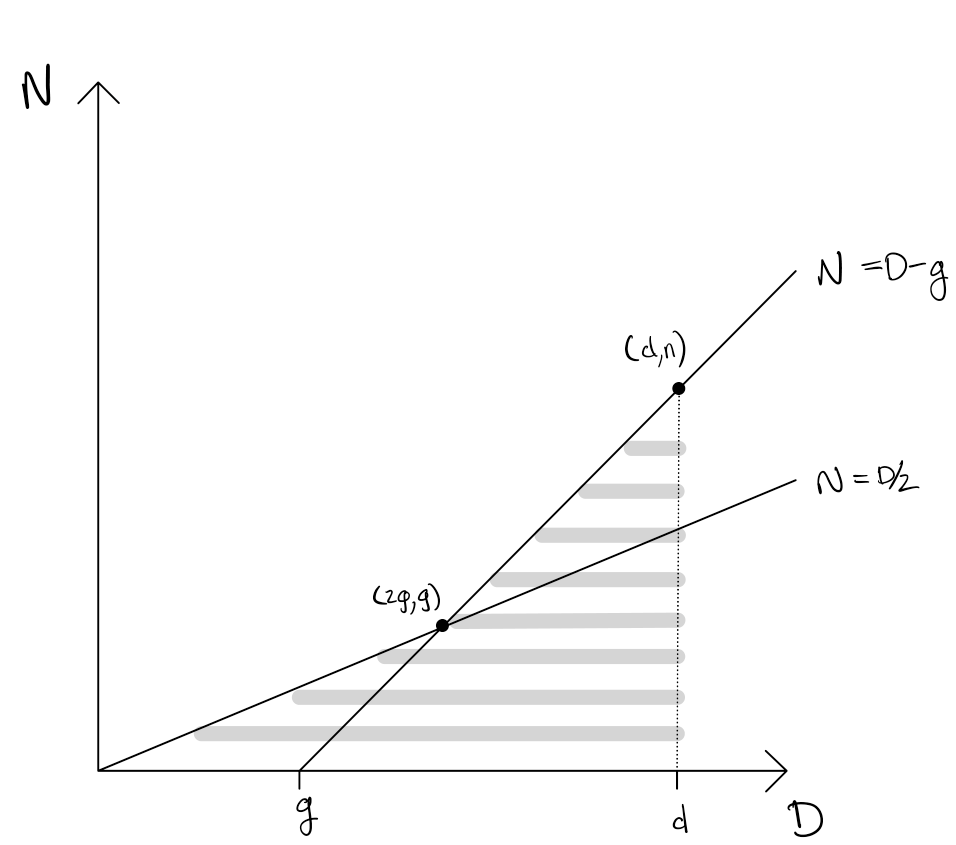
\includegraphics[width=.48\textwidth]{figures/fig-6.8.23.png}
\caption{到 $(d,\allowbreak n)$ 的直线斜率大于到阴影区域任何点的斜率.}\label{src:6.8.23}\end{figure}
对 (b), 选择坐标使单参数子群权满足 $\lambda_0\geq\cdots\geq\lambda_n=0$. 子空间 $\langle x_k,\allowbreak \ldots,\allowbreak x_n\rangle$ 定义超平面 $L_k=V(x_k,\allowbreak \ldots,\allowbreak x_n)$, 诱导到 $\mathbb P^{n-k}$ 的线性投影; $I_k$ 由这些坐标生成. 线性稳定性给出 $e_{\mathcal O_C(1)}(I_k)<(k/n)\deg C$. 命题~\bookref{6.8.19} 给出
\[
\begin{aligned}
e(C,\lambda)&\leq\sum_{k=0}^{n-1}(\lambda_k-\lambda_{k+1})\bigl(e_{\mathcal O_C(1)}(I_k)+e_{\mathcal O_C(1)}(I_{k+1})\bigr)\\
&<\frac{2\deg C}n\sum_{k=0}^{n-1}(\lambda_k-\lambda_{k+1})(k+\tfrac12)\\
&=\frac{2\deg C}n(\tfrac12\lambda_0+\lambda_1+\cdots+\lambda_{n-1}+\tfrac12\lambda_n)\\
&=\frac{2\deg C}n\Bigl(\sum_i\lambda_i-\tfrac12(\lambda_0+\lambda_n)\Bigr)\\
&\leq\frac{2\deg C}n\Bigl(\sum_i\lambda_i-\frac1{n+1}\sum_i\lambda_i\Bigr)
=\frac{2\deg C}{n+1}\sum_i\lambda_i.
\end{aligned}
\]
由 Chow 稳定性判据 (\bookref{6.8.17}) 得 Chow 稳定, 再由命题~\bookref{6.8.18} 得渐近 Hilbert 稳定.
\end{proof}
因此可推出光滑曲线的多重典范嵌入 Chow 稳定.
\begin{proof}[定理~\bookref{6.8.5}(1) 的证明]
嵌入 $|\omega_C^{\otimes k}|$ 的次数为 $d=2k(g-1)$, $N_k+1=(2k+1)(g-1)$. 若 $k\geq5$ (其实 $k\geq3$ 即可), 则 $d>2g$, 定理~\bookref{6.8.22} 给出 Chow 稳定和渐近 Hilbert 稳定. 进一步可找出充分大的 $m$, 使每条此类光滑曲线 $m$-Hilbert 稳定; 见~\cite[定理 1.0.0]{Gie82}.
\end{proof}
\begin{exercise}\label{src:6.8.24}
证明含结点的曲线 $C\subseteq\mathbb P^n$ 不线性稳定.
\end{exercise}
\begin{remark}\label{src:6.8.25}
有光滑曲面不 Chow 稳定, 例如映射 $\mathbb P^2\to\mathbb P^4$, $[x:y:z]\mapsto[xz:yz:x^2:xy:y^2]$ 的像定义的 Steiner 曲面~\cite[例 3.6]{Mor80}.
\end{remark}
\subsection{使非结点曲线去稳定化}\label{src:6.8.5-subsection}
\begin{proposition}\label{src:6.8.26}
设 $C\subseteq\mathbb P^n$ 一般约化, $\deg C/(n+1)<8/7$. 若 $C$ Chow 半稳定, 则不含于超平面, 且至多具有结点奇点.
\end{proposition}
\begin{proof}
若 $C\subseteq H$, 取坐标使 $H=V(x_0)$. 令 $\lambda(t)=\operatorname{diag}(t^{-n},\allowbreak t,\allowbreak \ldots,\allowbreak t)$, 指数严格为正, 所以非半稳定.

若 $p$ 为重数至少 $3$ 的奇点, 取 $p=(1,\allowbreak 0,\allowbreak \ldots,\allowbreak 0)$, $\lambda(t)=(t,\allowbreak 1,\allowbreak \ldots,\allowbreak 1)$. $J_\lambda=(tx_0,\allowbreak x_1,\allowbreak \ldots,\allowbreak x_n)$ 是 $(0,\allowbreak p)$ 的极大理想, 且
\[
e(C,\lambda)=\operatorname{mult}_{(0,p)}(\mathbb A^1\times C)
=\operatorname{mult}_p C\geq3>\frac{16}7\sum_i\lambda_i
>\frac{2\deg C}{n+1}\sum_i\lambda_i.
\]
由判据非半稳定.

若 $p$ 是非结点的二重点, 令 $L\subseteq\mathcal O_C$ 定义 $p$ 处的约化切线. 则 $\mathfrak m_p^2\subsetneq\mathfrak m_p^2+L\subsetneq\mathfrak m_p$, 且 $\dim_k\mathfrak m_p/\mathfrak m_p^2=2$. 取坐标使 (i) $x_0(p)\ne0$, (ii) $v=x_1/x_0$, $u=x_2/x_0$ 张成该商, (iii) $u\in L$, $u^2\in\mathfrak m_p^3$, (iv) $x_3/x_0,\allowbreak \ldots,\allowbreak x_n/x_0\in\mathfrak m_p^2$. 置 $\lambda(t)=\operatorname{diag}(t^4,\allowbreak t^2,\allowbreak t,\allowbreak 1,\allowbreak \ldots,\allowbreak 1)$, 则 $J_\lambda$ 定义支撑在 $(0,\allowbreak p)$ 的闭子概形. 所以 $e(C,\allowbreak \lambda)=e(J_\lambda)$ 是 Hilbert--Samuel 重数, 无论用 $\mathcal O_{\mathbb A^1}\boxtimes\mathcal O_C(1)$ 还是结构层计算均相同. 置 $J_0=(t^4,\allowbreak t^2v,\allowbreak tu,\allowbreak \mathfrak m_p^2)$, 则 $J_\lambda\subseteq J_0$, $e(J_\lambda)\geq e(J_0)$. 令 $J_1=(t^4,\allowbreak \mathfrak m_p^2)$. 因为
\[
(t^2v)^2=t^4v^2\in J_1^2,\qquad
(tu)^4=t^4(u^2)^2\in t^4(\mathfrak m_p^3)^2\subseteq J_1^4,
\]
对 $m\gg0$, $J_0^m=J_1^m$, 所以 $e(J_0)=e(J_1)$. 因而
\[
\begin{aligned}
e(C,\lambda)&=e(J_\lambda)\geq e(J_0)=e(J_1)
=4\cdot2\cdot\operatorname{mult}_p C=16\\
&=\frac{16}7\sum_i\lambda_i>\frac{2\deg C}{n+1}\sum_i\lambda_i.
\end{aligned}
\]
再次由判据得非半稳定. 另见~\cite[命题 3.1]{Mum77} 和~\cite[命题 1.0.4]{Gie82}.
\end{proof}
\begin{remark}\label{src:6.8.27}
有些低次数 Chow 稳定曲线具有比结点更严重的奇点, 但以更高次数重新嵌入后会非半稳定. 例如有次数 $4$ 的 Chow 稳定尖点曲线 $C\subseteq\mathbb P^2$ (见习题~\bookref{8.5.4}), 以次数 $8$ 的线丛 $\mathcal O_C(2)$ 重新嵌入后却非半稳定.
\end{remark}
\begin{proof}[定理~\bookref{6.8.5}(2) 的证明]
若 $C$ 为 $k\geq5$ 的多重典范嵌入稳定曲线, 则
\[
\frac{\deg C}{n+1}=\frac{2k(g-1)}{(2k-1)(g-1)}=\frac{2k}{2k-1}<\frac87.
\]
故命题~\bookref{6.8.26} 保证一般约化且 Chow 半稳定的 $C$ 不含于超平面, 至多具有结点奇点. 要进一步排除非一般约化或非 $k$-多重典范嵌入的曲线, 需相当长而细致的去稳定化分析; 细节见~\cite[\S5]{Mum77}, \cite[\S1]{Gie82} 和~\cite[定理 4.45]{HM98}.
\end{proof}
